\documentclass{article}

\usepackage{graphicx}
\usepackage{fancyhdr}
\usepackage[sorting=none]{biblatex}
\usepackage[margin=1in]{geometry}
\usepackage{listings}
\usepackage{float}
\usepackage{hyperref}
\usepackage{xepersian}

\addbibresource{bibliography.bib}
\settextfont[Scale=1.2]{B-NAZANIN.TTF}
\setlatintextfont[Scale=1]{Times New Roman}
\renewcommand{\baselinestretch}{1.5}
\pagestyle{fancy}
\fancyhf{}
\rhead{تکلیف اول درس سیستم‌های عامل 1 }
\lhead{\thepage}
\rfoot{علیرضا ابره فروش}
\lfoot{9816603}
\renewcommand{\headrulewidth}{1pt}
\renewcommand{\footrulewidth}{1pt}

%%%%%%%%%%%%%%%%
\setcounter{secnumdepth}{3}
\setcounter{tocdepth}{3}
%%%%%%%%%%%%%%%%
\begin{document}
\begin{titlepage}
\begin{center}

\includegraphics[width=0.4\textwidth]{figures/IUT Logo.png}\\
        
\LARGE
\textbf{دانشگاه صنعتی اصفهان}\\
\textbf{دانشکده مهندسی برق و کامپیوتر}\\
        
\vfill
        
\huge
\textbf{عنوان: تکلیف چهارم درس ریزپردازنده}\\
        
\vfill
        
\LARGE
\textbf{نام و نام خانوادگی: علیرضا ابره فروش}\\
\textbf{شماره دانشجویی: 9816603}\\
\textbf{نیم\,سال تحصیلی: پاییز 1400}\\
\textbf{مدرّس: دکتر عارف کریمی افشار}\\
\end{center}
\end{titlepage}


\tableofcontents
\newpage

\section{عنوان سوال اول}
اگر سوال بخش\,بندی\,شده نباشد، پاسخ آن در این قسمت نوشته می\,شود.
\subsection{عنوان بخش اول سوال اول}
پاسخ بخش اول سوال در این قسمت نوشته می\,شود.
\subsection{عنوان بخش دوم سوال اول}
پاسخ بخش دوم سوال در این قسمت نوشته می\,شود.
\subsection{عنوان بخش سوم سوال اول}
پاسخ بخش دوم سوال در این قسمت نوشته می\,شود.
\subsection{عنوان بخش چهارم سوال اول}
محتوای برخی از رجیستر‌ها مانند \lr{Program Counter} یا \lr{Stack Pointer} توسط \lr{kernel handler} قابل ذخیره‌سازی نیستند. چون خود آن‌ها هم نرم‌افزار هستند و تا \lr{CPU} بخواهد آن‌ها را وارد مرحله اجرا کند، محتوای \lr{Program Counter} و \lr{Stack Pointer} عوض می‌شود. پس سخت افزار قبل از فراخوانی  \lr{kernel handler}، به طور خودکار محتوای رجیستر‌های برخی از پروسس‌های متوقف شد را با \lr{push} کردن آن‌ها در \lr{interrup stack} حفظ می‌کند.
\subsection{عنوان بخش پنجم سوال اول}
پاسخ بخش دوم سوال در این قسمت نوشته می\,شود.
\subsection{عنوان بخش ششم سوال اول}
پاسخ بخش دوم سوال در این قسمت نوشته می\,شود.
\subsection{عنوان بخش هفتم سوال اول}
پاسخ بخش دوم سوال در این قسمت نوشته می\,شود.

\section{عنوان سوال دوم}
\indent
سیستم کال \lr{fork()} یک پروسس جدید به نام پروسس \lr{child} می‌سازد. پس از ایجاد پروسس \lr{child}، هر دو پروسس(\lr{child} و \lr{parent}ش)دستوراتی که پس از \lr{fork()} متناظرشان آمده اند را یک به یک اجرا می‌کنند. به این ترتیب پس از اولین \lr{fork()}، در مجموع 2 پروسس، پس از دومین \lr{fork()}، در مجموع 4 پروسس، پس از سومین \lr{fork()}، در مجموع هشت پروسس و $\ldots$، خواهیم داشت. درنتیجه پس از اجرای حلقه، تعداد \lr{child}های ایجاد شده برابر است با:

\begin{center}
$
2+4+\ldots+2^{\log_2 n}=2^{(\log_2 n)+1}=2n
$
\end{center}
در مجموع با احتساب پروسس \lr{parent} اصلی، \lr{n}2 پروسس خواهیم داشت.

\section{عنوان سوال سوم}
در این قسمت با نحوه درج روابط و فرمول\,ها آشنا می\,شوید:
\begin{center}
$E = m{c}^{2}$
\end{center}

\section{عنوان سوال چهارم}
یک راه این است که مقدار رجیستری که به جدول وقفه(\lr{Interrupt Vector Table}) اشاره می‌کند را عوض کنیم. درواقع می‌توانیم مکان دلخواهی از حافظه را به عنوان مکان جدول وقفه مشخص کنیم. توسط دستور \lr{lidt} در \lr{x86} می‌توان این رجیستر را مقداردهی کرد. بنابراین این دستور است که مشخص می‌کند که این جدول کجای حافظه قرار گرفته است. بدیهی است که تنها سیستم عامل باید دسترسیِ استفاده از این دستور را داشته باشد. در غیراینصورت، اگر پروسسی بتواند از این دستور استفاده کند، می‌تواند هر کاری را روی سیستم انجام دهد. چون می‌تواند جدول وقفه را طبق نظر خودش تنظیم کند و سپس آدرس حافظه‌ای که به ابتدای آن جدول اشاره می‌کند را در داخل آن رجیستر خاص توسط دستور \lr{lidt} ثبت کند و در نتیجه بسیاری از مفاهیم و سرویس‌هایی که در مورد سیستم عامل مد نظر داشتیم نقض می‌شود.
\lr{\lstinputlisting[language=C, showstringspaces=false, basicstyle=\ttfamily]{sources/lidt.c}}
\begin{figure}[H]
    \centering
    
\includegraphics[width=0.8\textwidth]{figures/4.png}
    \caption{خطای رخ داده پس از اجرای برنامه}
    \label{fig:fig1}
\end{figure}
با اجرای برنامه بالا مشاهده می‌شود که \lr{Segmentation fault (core dumped)} رخ می‌دهد. \lr{segmentation fault} یک خطا است که توسط سخت‌افزار در راستای \lr{memory protection}، به سیستم عامل اطلاع می‌دهد که یک برنامه تلاش کرده است که به یک بخش حفاظت شده از حافظه دسترسی پیدا کند(\lr{a memory access violation}). در کامپیوترهای استاندارد \lr{x86}، این یک فرم از \lr{general protection fault} است.

\section{عنوان سوال پنجم}
\subsection{}
\lr{\lstinputlisting[language=C, showstringspaces=false, basicstyle=\ttfamily]{sources/collatz_conjecture.c}}
\subsection{}
زیرا در \lr{UNIX/POSIX}، \lr{exit code}ِ یک برنامه از نوع \lr{unsigned 8-bit} تعریف شده است. به طور دقیق‌تر \lr{system call}های خانواده \lr{wait} در \lr{UNIX} نتیجه یک پروسس را به یک \lr{32-bit integer} کدگذاری می‌کنند. از این 32 بیت برای اطلاعاتی همچون وقوع یا عدم وقوع \lr{dump core} در پروسس، \lr{exit} به دلیل یک سیگنال(و چه سیگنالی)، و $\ldots$ تقسیم می‌شود. از این رو تنها 8 بیت از 32 بیت برای \lr{exit code} باقی می‌ماند. پس در نتیجه مقادیر 0 تا 255 به این شکل قابل برگردانده شدن هستند.

\subsection{}


\section{عنوان سوال ششم}
\subsection{}
\textbf{\lr{orphan process}:}
پروسسی که \lr{parent}ش وجود ندارد(یا پایان یافته یا بدون اینکه برای متوقف شدن \lr{child}ش صبر کرده باشد، متوقف شده باشد)، \lr{orphan process} نامیده می‌شود.
\newline
\textbf{\lr{zombie process}:}
پروسسی که اجرای آن پایان یافته است اما هنوز در جدول پروسس‌ها مقداری دارد که به پروسس \lr{parent} نسبت داده می‌شود، \lr{zombie process} نامیده می‌شود. یک پروسس \lr{child} همواره پیش از پاک شدن از جدول پروسس‌ها به یک \lr{zombie process} تبدیل می‌شود. پروسس \lr{parent}، \lr{exit status} پروسس \lr{child} را می‌خواند و پروسس \lr{child} از جدول پروسس‌ها حذف می‌شود.
\subsection
\indent
برنامه‌ی 1 یک \lr{orphan process} ایجاد می‌کند. چون پروسس \lr{child} حدودا 101 ثانیه پس از پایان یافتن پروسس \lr{parent} به پایان می‌رسد. همینطور که در تصویر اول مشهود است، مقدار \lr{ppidِ}ِ پروسس \lr{child} پس از ثانیه اول برابر 2174(\lr{pidِ}ِ پروسس \lr{parent}) است اما پس از ثانیه سوم(پایان یافتن پروسس \lr{parent}) این مقدار برابر 1286(\lr{pid}ِ پروسس \lr{systemd} که نقش \lr{subreaper} را برای پروسس \lr{orphan} برعهده دارد و در قسمت بالای جدول پروسس‌ها قرار دارد) می‌باشد.
\begin{figure}[H]
    \centering
    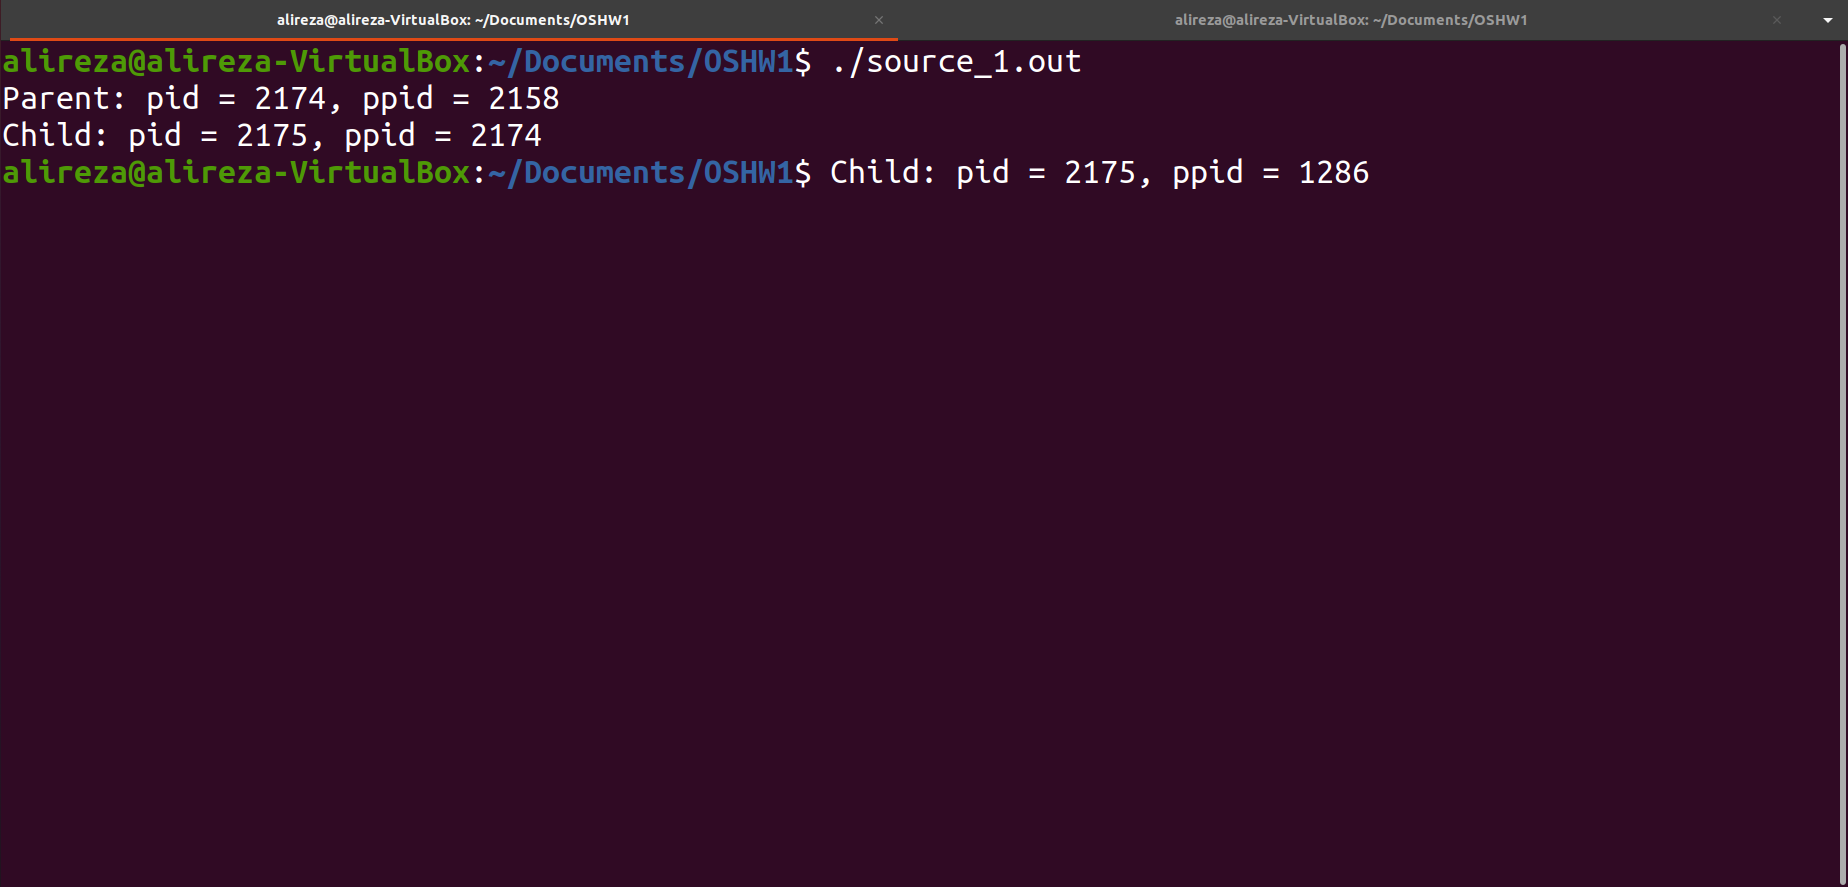
\includegraphics[width=0.8\textwidth]{figures/6.2.1.1.png}
    \caption{اجرای برنامه‌ی 1}
    \label{fig:fig1}
\end{figure}

\begin{figure}[H]
    \centering
    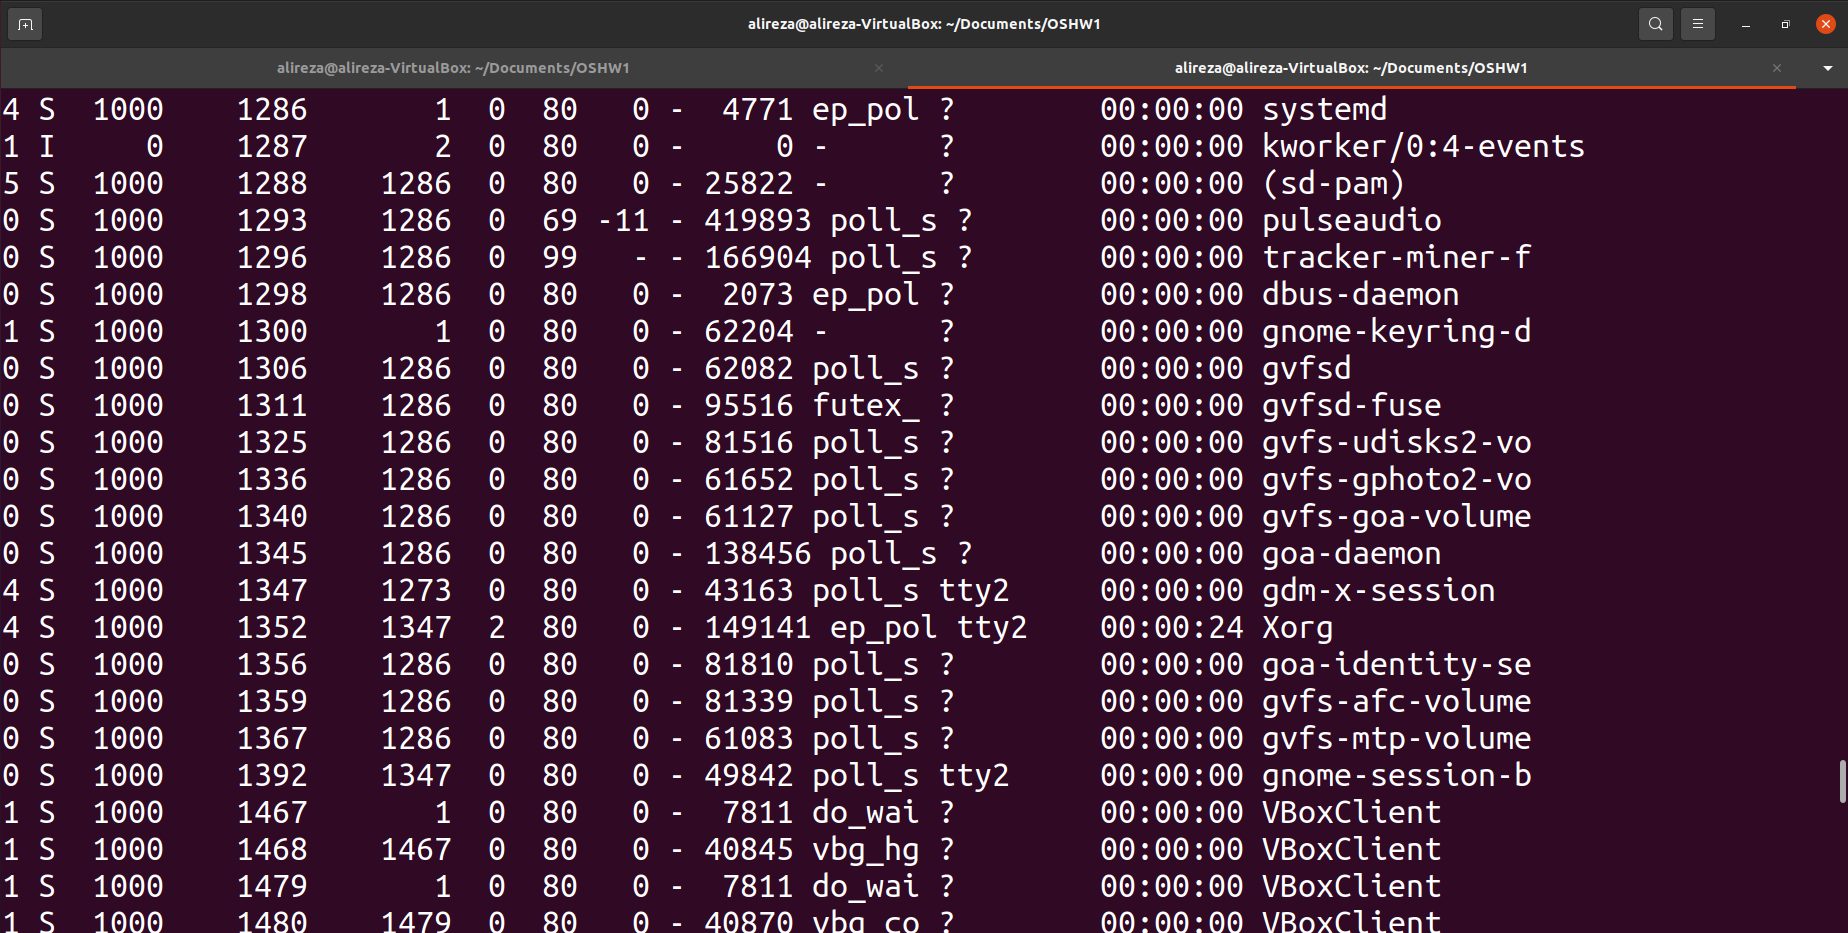
\includegraphics[width=0.8\textwidth]{figures/6.2.1.3.png}
    \caption{جدول پروسس‌ها(قسمت بالا)}
    \label{fig:fig1}
\end{figure}

\begin{figure}[H]
    \centering
    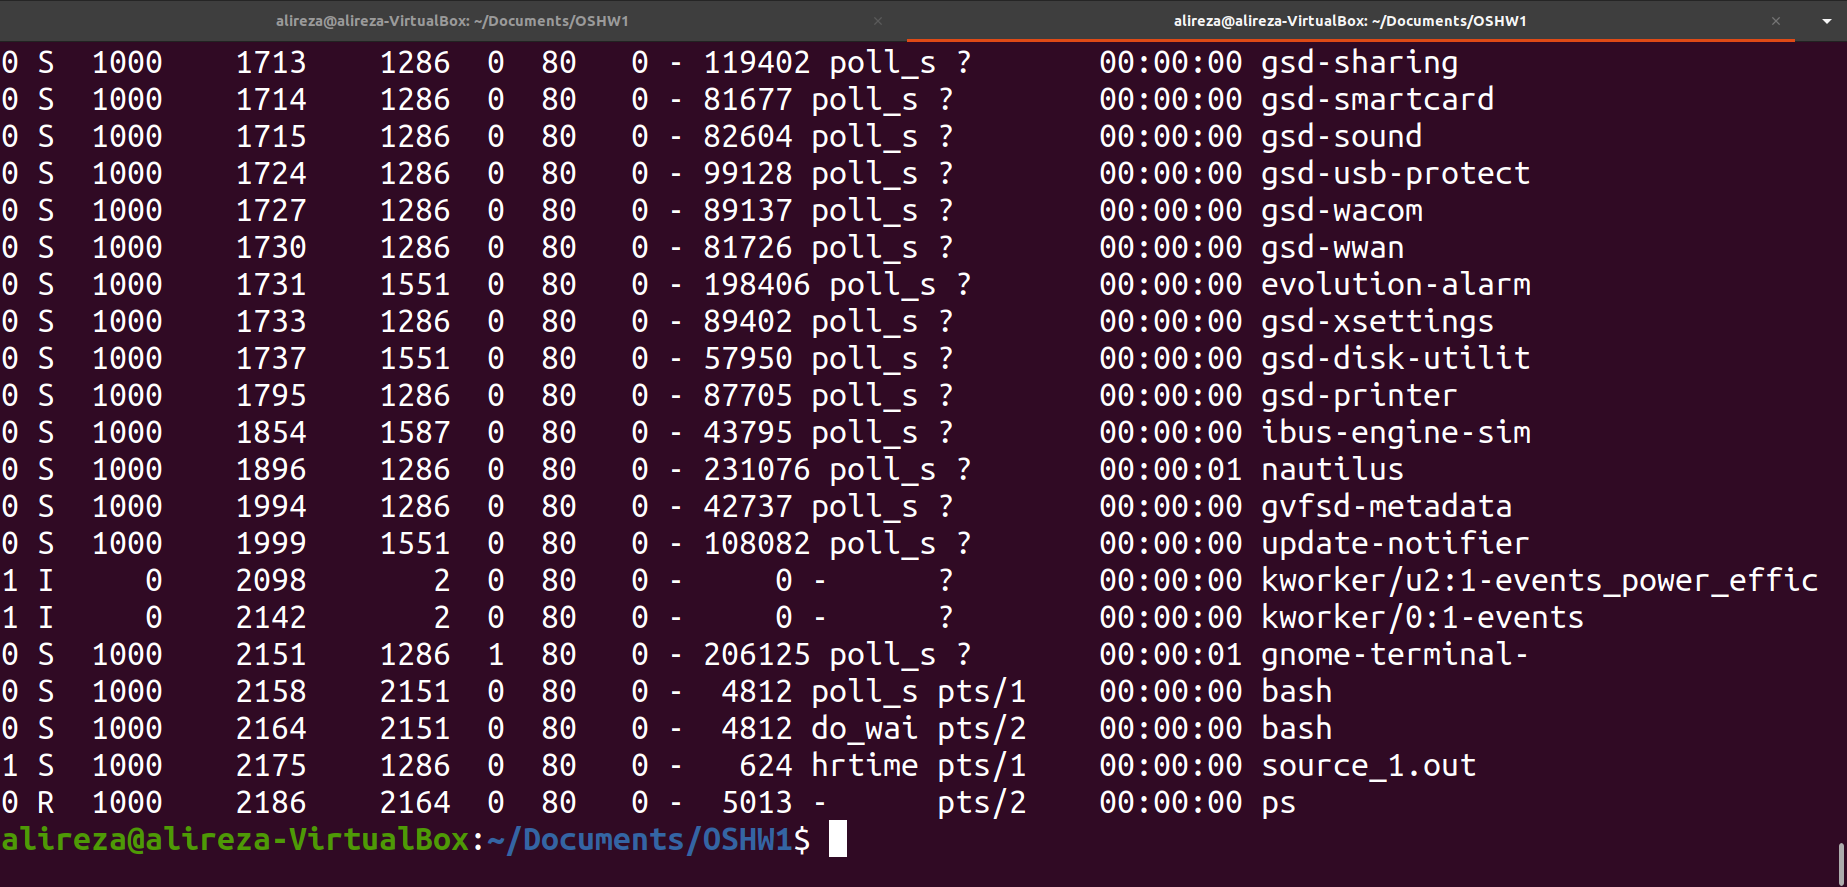
\includegraphics[width=0.8\textwidth]{figures/6.2.1.2.png}
    \caption{جدول پروسس‌ها(قسمت پایین)}
    \label{fig:fig1}
\end{figure}
%%%%%%%%%%%%%

برنامه‌ی 2 یک \lr{zombie process} ایجاد می‌کند. چون پروسس \lr{parent} حدودا 99 ثانیه پس از پایان یافتن پروسس \lr{child} به پایان می‌رسد. اگر در این بازه زمانی جدول پروسس‌ها را بررسی کنیم می‌بینیم که پروسسی با \lr{STAT}ِ \lr{Z} وجود دارد که \lr{pid}ش برابر \lr{pid}ِ پروسس \lr{child} است و این نشان‌دهنده این است که برنامه‌ی 2 یک \lr{zombie process} تولید کرده است. به تصاویر زیر توجه کنید:
\begin{figure}[H]
    \centering
    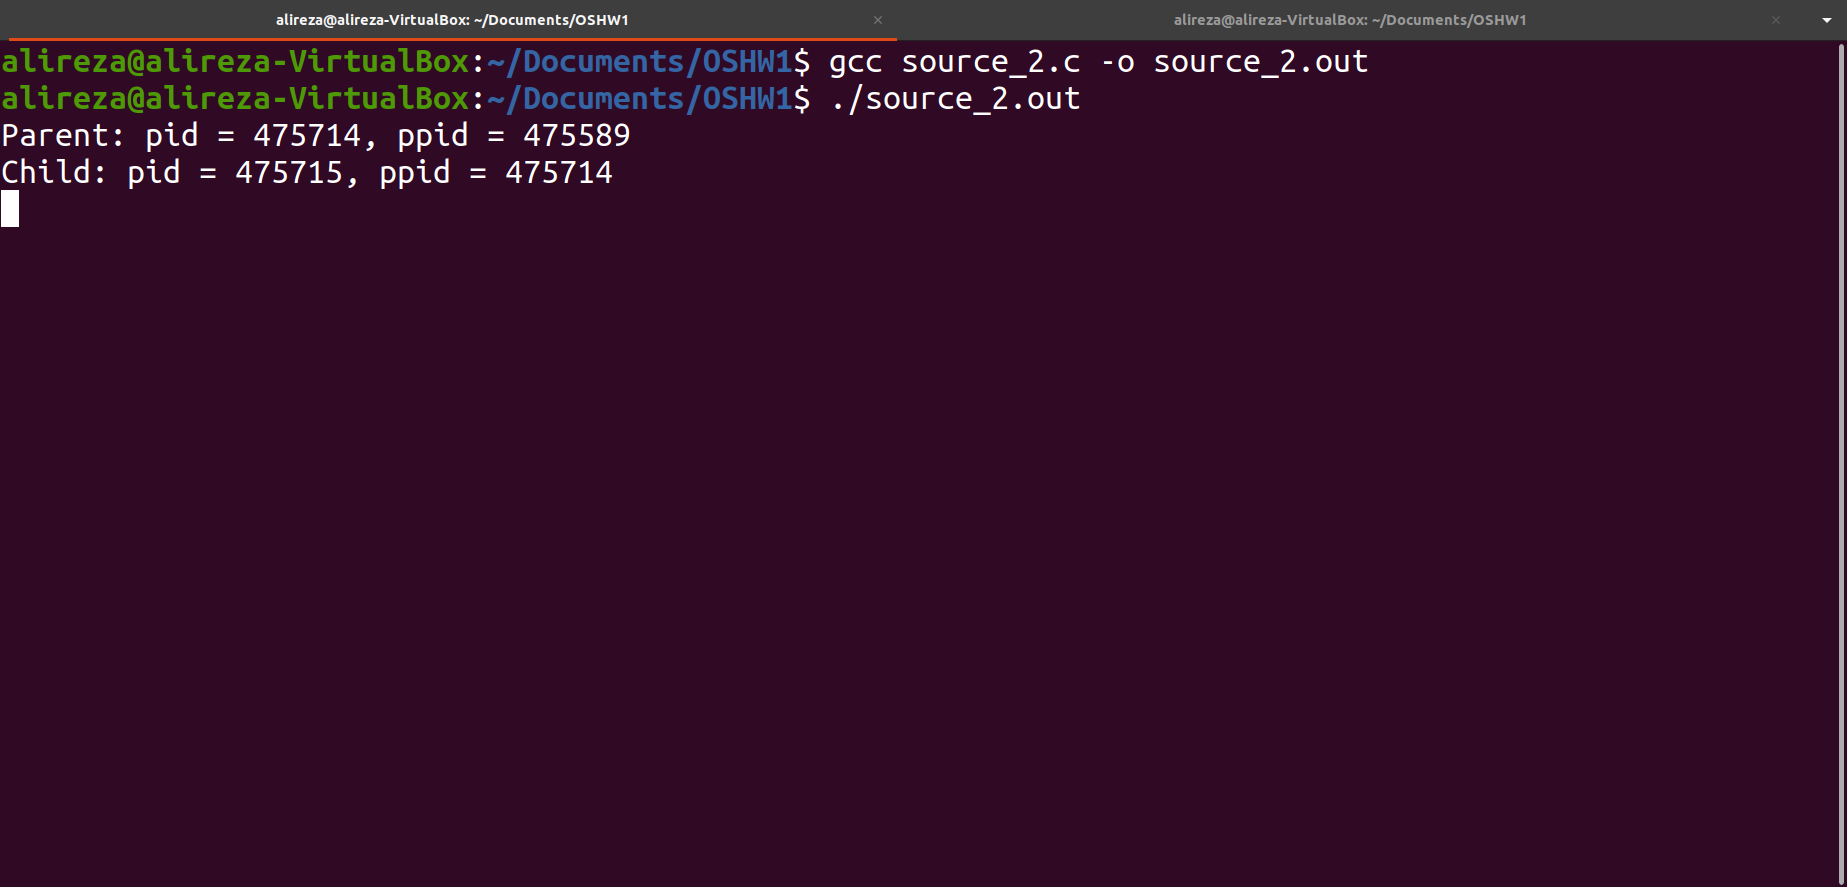
\includegraphics[width=0.8\textwidth]{figures/6.2.2.1.png}
    \caption{اجرای برنامه‌ی 2}
    \label{fig:fig1}
\end{figure}

\begin{figure}[H]
    \centering
    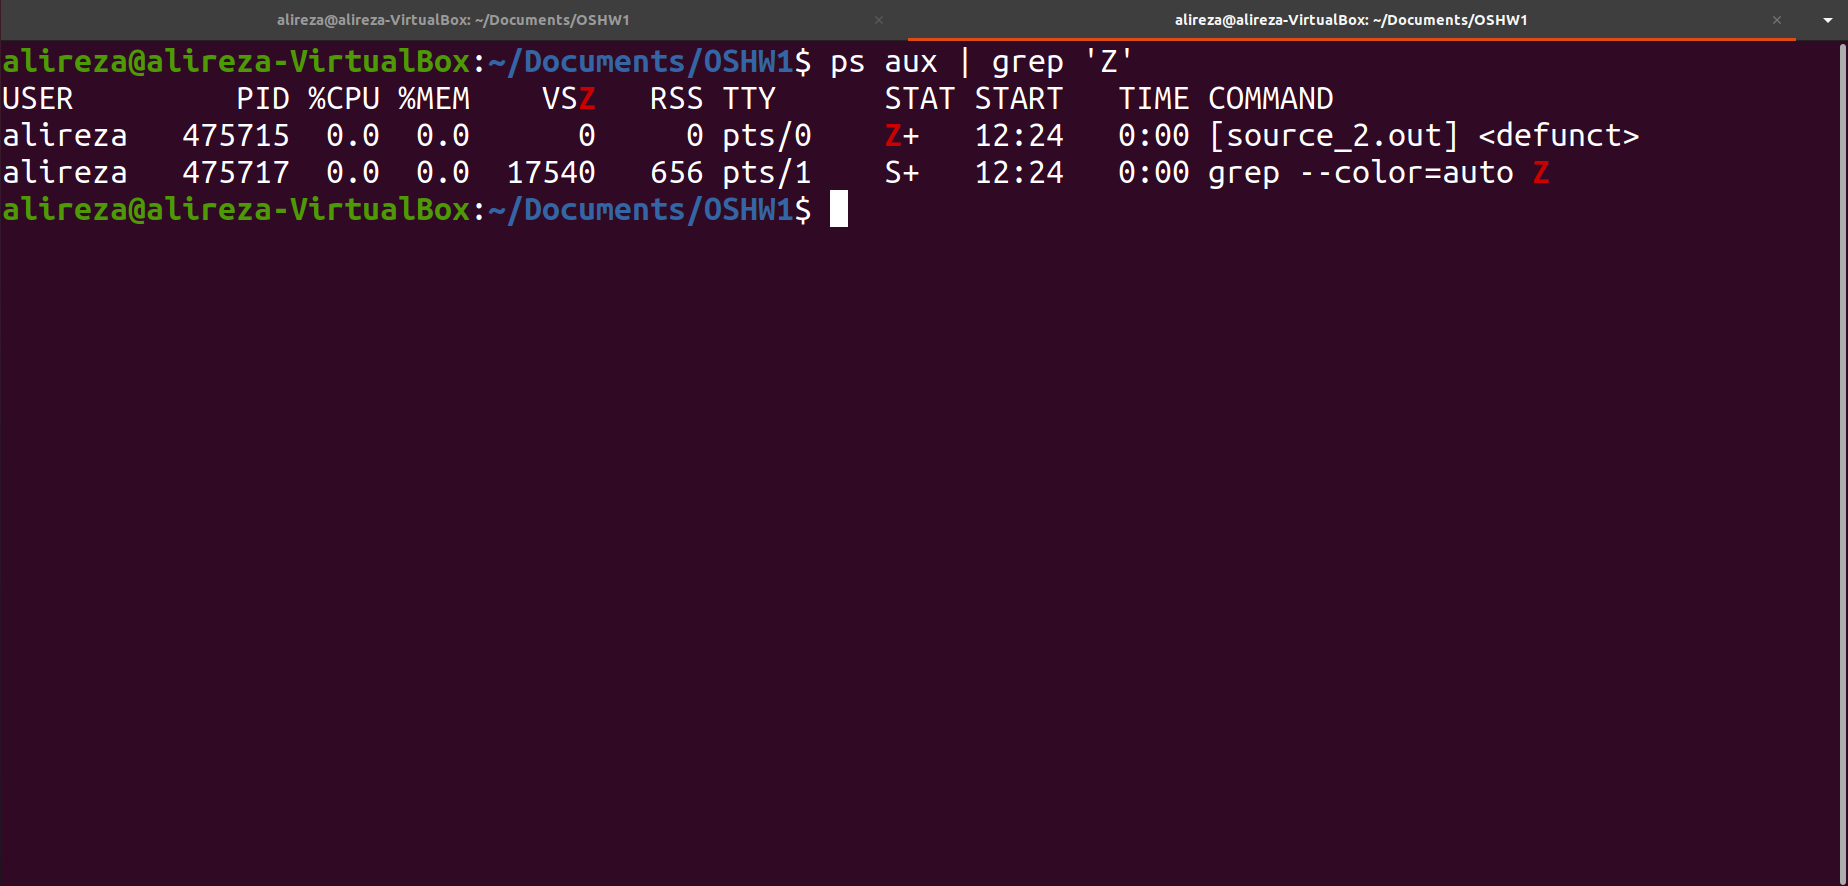
\includegraphics[width=0.8\textwidth]{figures/6.2.2.2.png}
    \caption{جدول پروسس‌ها}
    \label{fig:fig1}
\end{figure}

\section{سوال هفتم}
\subsection{سوال 6 فایل}
با اجرای دستور سوال، یک پروسه دارای 3 دستور که از \lr{IOs} و سه پروسه هر کدام دارای 5 دستور که از \lr{CPU} استفاده می‌کنند برای اجرا آماده می‌شوند.
\newline
خیر-منابع به طور موثر و بهینه به کار گرفته نشده‌اند. همانطور که در تصویر اول می‌بینیم \lr{IOs} در بازه‌ی زمانی 7 تا 18 و همچنین \lr{CPU} در بازه‌ی زمانی 19 تا 23 و 26 تا 30 بی‌کار هستند و درنهایت در 31 واحد زمانی \lr{CPU} تنها 67/74 درصد مواقع، و \lr{IOs} تنها 48/39 درصد مواقع مشغول بوده‌اند. به عبارت دیگر در 31 واحد زمانی، \lr{CPU}، 21 واحد زمانی و \lr{IOs}، 15 واحد زمانی درحال استفاده بوده‌اند.
\begin{figure}[H]
    \centering
    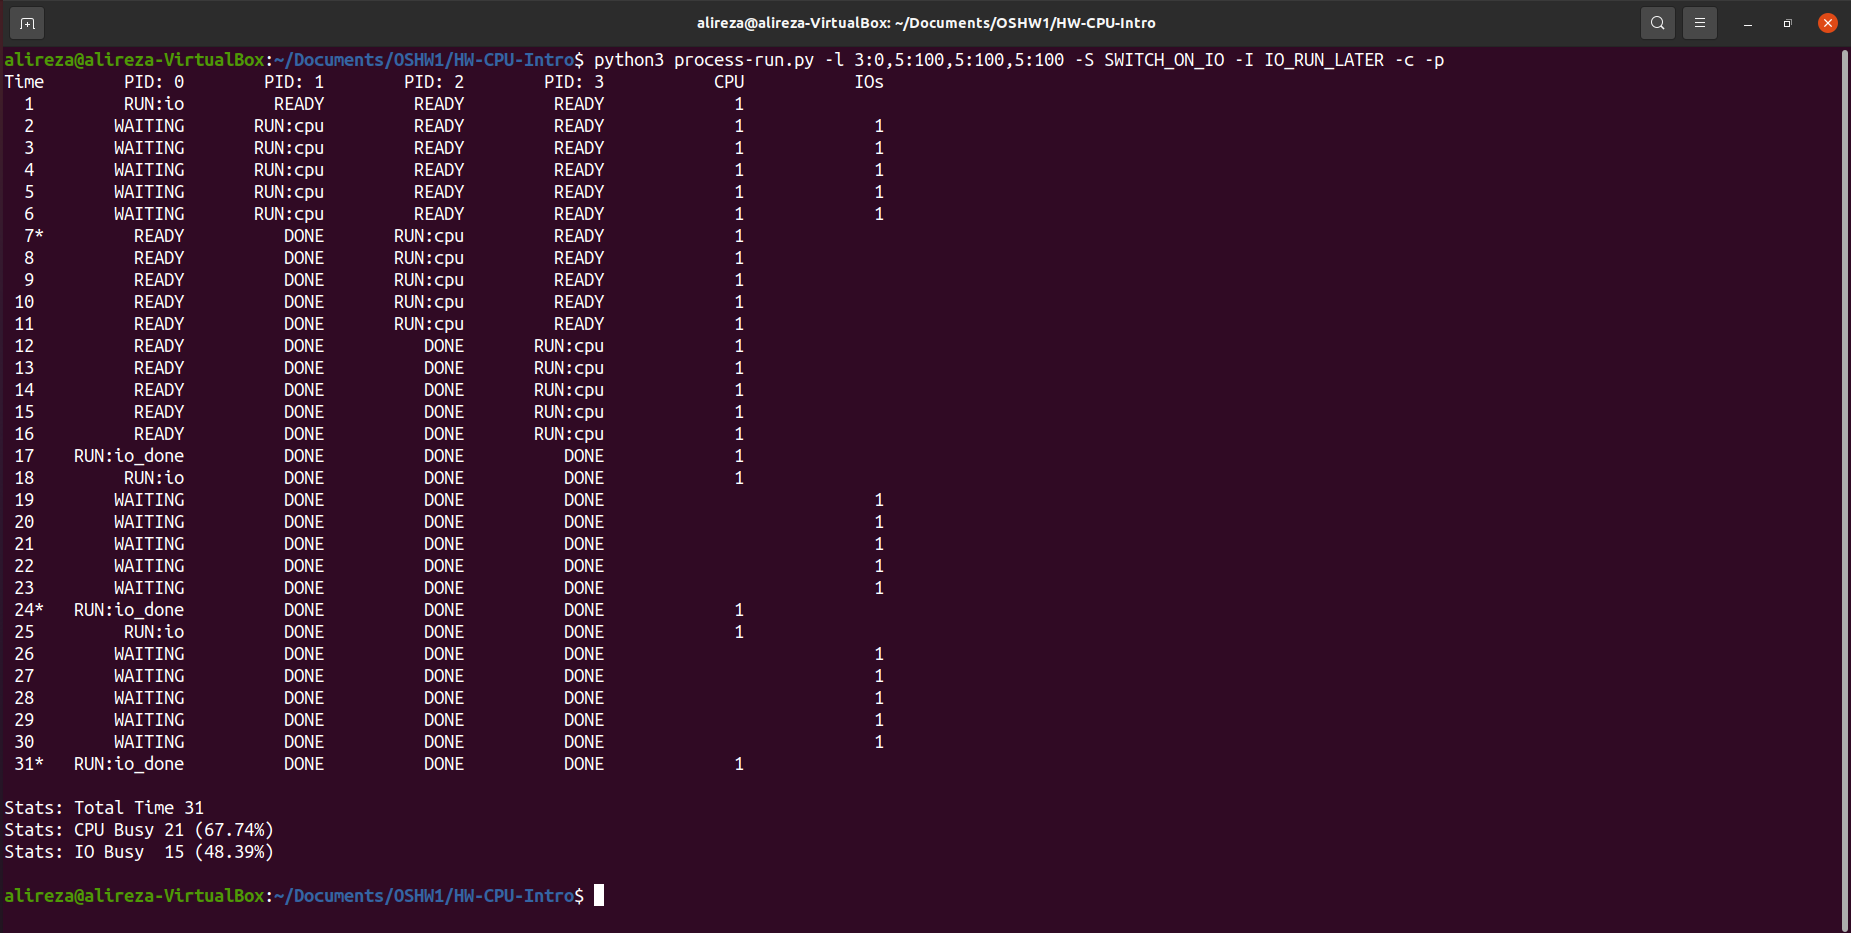
\includegraphics[width=0.8\textwidth]{figures/7.1.png}
    \caption{}
    \label{fig:fig1}
\end{figure}
\subsection{سوال 7 فایل}
تفاوتی که این حالت با حالت قبل دارد این است که عملکرد \lr{CPU} و \lr{IOs} در بازه‌های بیشتری همزمان به موازات یکدیگر رخ می‌دهند. درواقع در این حالت پس از پایان یافتن \lr{IO}، بلافاصله به این پروسس سوئیچ می‌کند و درنتیجه 5 دستور اجرای \lr{IO}(\lr{waiting})، با 5 دستور اجرای \lr{CPU} موازی می‌شود. با دقت در تصویر دوم می‌بینیم که زمان کل به 21 واحد کاهش یافته است، \lr{CPU} در کلِ 21 واحد مشغول بوده است، و \lr{IOs} نیز در 15 واحد درحال استفاده بوده است(درست است که در هر دو حالت، \lr{IOs} در 15 واحد زمانی استفاده شده است، اما در حالت قبل، \lr{IOs} تنها در 48/39 درصد مواقع مشغول بوده است، درحالی که در این حالت در 71/43 درصد مواقع درحال استفاده بوده است. پس در این سوال با شرایط ذکر موجود، اجرای بلافصل پروسسی که اخیرا \lr{I/O}ی آن کامل شده است ایده خوبی می‌تواند باشد.
\begin{figure}[H]
    \centering
    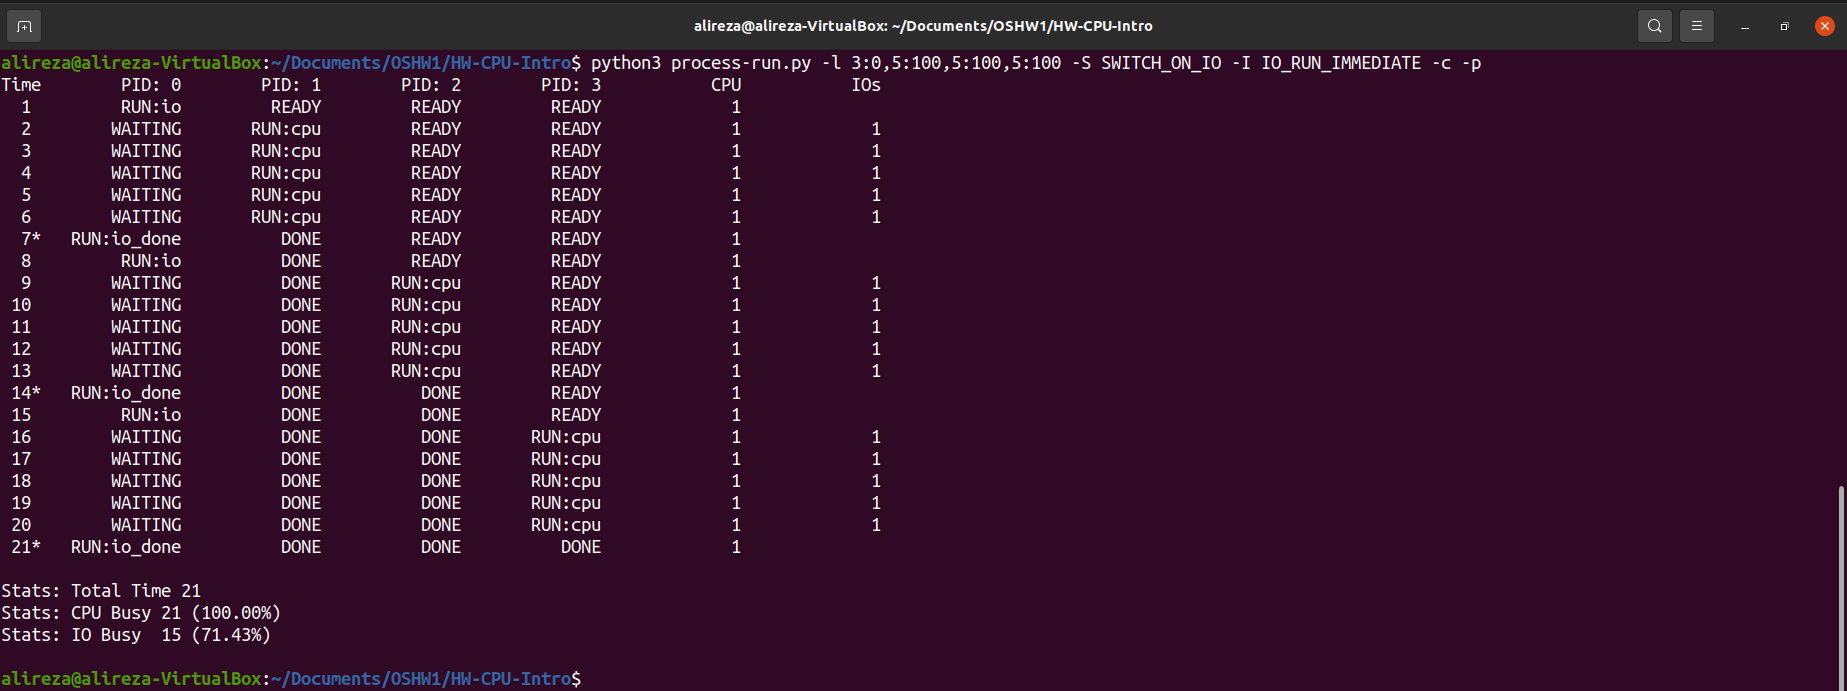
\includegraphics[width=0.8\textwidth]{figures/7.2.png}
    \caption{}
    \label{fig:fig1}
\end{figure}
%%%%%%%%%%%%%%%%%%%%%%%%%%%%%%%
\section{عنوان سوال جدول}
در این قسمت با نحوه درج جداول آشنا می\,شوید:
\begin{table}[ht]
    \centering
    \begin{tabular}{|c|c|c|}
    \hline
    خانه شماره 1 & خانه شماره 2 & خانه شماره 3\\
    \hline
    خانه شماره 4 & خانه شماره 5 & خانه شماره 6\\
    \hline
    خانه شماره 7 & خانه شماره 8 & خانه شماره 9\\
    \hline
    \end{tabular}
    \caption{جدول شماره 1}
    \label{tab:tab1}
\end{table}

%%%%%%%%%%%%%%%%%%%%%%%%%%%%%%%


\section{عنوان سوال هشتم}
در این قسمت با نحوه ارجاع به سایر منابع آشنا می\,شوید:\\
\indent
به صفحه درس سیستم عامل دکتر محمّدرضا حیدرپور ارجاع داده می\,شود \cite{b1}.

\section{ضمیمه}
برای آشنایی بیشتر با \lr{\LaTeX}، با جست\,و\,جو در اینترنت منابع مفیدی خواهید یافت.

%\printbibliography[title=منابع]

\section*{منابع}
\renewcommand{\section}[2]{}%
\begin{thebibliography}{99} % assumes less than 100 references
%چنانچه مرجع فارسی نیز داشته باشید باید دستور فوق را فعال کنید و مراجع فارسی خود را بعد از این دستور وارد کنید


\begin{LTRitems}

\resetlatinfont

\bibitem{b1} http://mrheidar.ir/courses/operating\_system.html
\end{LTRitems}

\end{thebibliography}


\end{document}
